\documentclass{bmvc2k}
\usepackage{amsfonts}
\usepackage{booktabs}
\usepackage{amsmath}
\usepackage{amssymb}
\usepackage{bbm}
\usepackage{bm}

%% Enter your paper number here for the review copy
\bmvcreviewcopy{611}

\title{Probabilistic Object Reconstruction with Online Loop Closure - Supplementary Material}

% Enter the paper's authors in order
% \addauthor{Name}{email/homepage}{INSTITUTION_CODE}
\addauthor{Jack Hunt}{jack.hunt@eng.ox.ac.uk}{1}
\addauthor{Victor Prisacariu}{victor.prisacariu@eng.ox.ac.uk}{1}
\addauthor{Stuart Golodetz}{stuart.golodetz@eng.ox.ac.uk}{1}
\addauthor{Philip Torr}{philip.torr@eng.ox.ac.uk}{1}

% Enter the institutions
% \addinstitution{Name\\Address}
\addinstitution{
 Department of Engineering Science\\
 University of Oxford,
 Parks Road, Oxford, OX1 3PJ
}

\runninghead{Student, Prof, Collaborator}{BMVC Author Guidelines}

% Any macro definitions you would like to include
% These are not defined in the style file, because they don't begin
% with \bmva, so they might conflict with the user's own macros.
% The \bmvaOneDot macro adds a full stop unless there is one in the
% text already.
\def\eg{\emph{e.g}\bmvaOneDot}
\def\Eg{\emph{E.g}\bmvaOneDot}
\def\etal{\emph{et al}\bmvaOneDot}

%------------------------------------------------------------------------- 
% Document starts here
\begin{document}

\maketitle

\section{Segmentation Model Details}
The segmentation model from which the probability maps are derived is an on-line Random Forest trained on patch features. 
The patch features are derived from the RGB and depth frames, incorporating information such as colour, depth, colour gradients and depth gradients.
In some of our experiments however, slightly better segmentation quality(qualitatively) has been achieved using features from a Deep Residual Neural Network \cite{residualNets}.
Such is the case for the \textit{DinoHead} and \textit{Rock} sequences.

Every $n$ frames the on-line Random Forest is trained with the mask for the current frame used to determine the positive/negative class training instances.
In our experiments $n = 10$.

\section{Comparison with Ren et al}
In the main paper a comparison is drawn on the reconstruction efficacy of our method versus that of Ren et al \cite{Ren2013} using a large shape prior. In figure \ref{fig:dinoComparison} 
we demonstrate the systems lack of ability to converge to a reasonable shape given a smaller shape prior.

\begin{figure}[!h]
	\centering
	\begin{tabular}{cc}
		\bmvaHangBox{\fbox{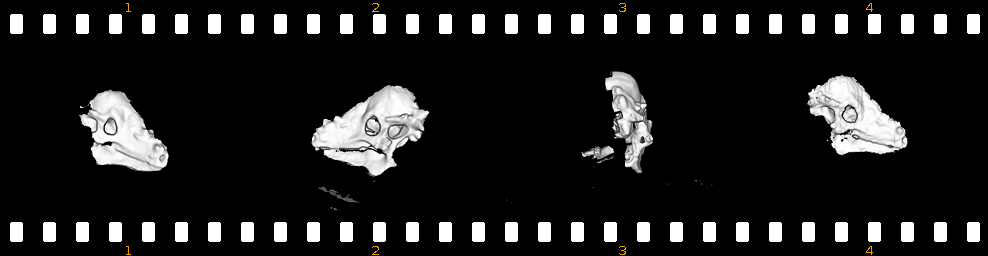
\includegraphics[width=0.45\textwidth]{filmstrips/dino.png}}}&
		\bmvaHangBox{\fbox{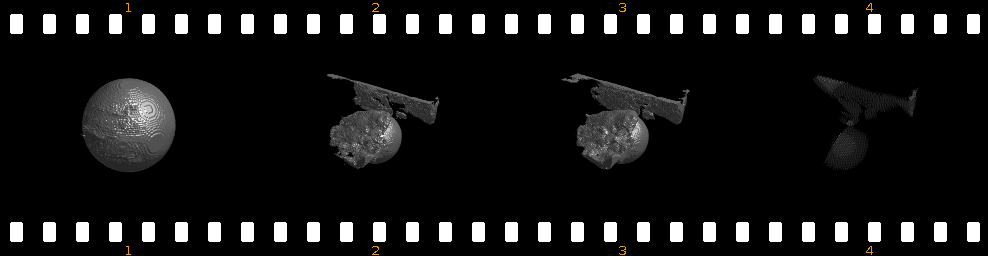
\includegraphics[width=0.45\textwidth]{filmstrips/dino_s3d_small.png}}}
	\end{tabular}
	\caption{
		Quarterly interval snapshots of the Dinosaur Head reconstruction using \textbf{(L)} our method, and \textbf{(R)} the one proposed by Ren et~al.~\cite{Ren2013} with a small shape prior.
	}
	\label{fig:dinoComparison}
\end{figure}

In addition to the comparisons between our method and that of \cite{Ren2013} on the \textit{DinoHead} sequence we also provide quarterly reconstruction snapshots on the \textit{Rock} 
sequence. Similar performance may be seen in figure \ref{fig:rockComparisonLarge} for a large shape prior and in figure \ref{fig:rockComparisonSmall} for a small shape prior.
It should be noted that although results from the system of Ren et al \cite{Ren2013} have been presented for two of the sequences our system was tested on, the results for the 
remaining sequences were very similar. We were unable to reconstruct any of our test objects with the system of Ren et al \cite{Ren2013}.

\begin{figure}[!h]
	\centering
	\begin{tabular}{cc}
		\bmvaHangBox{\fbox{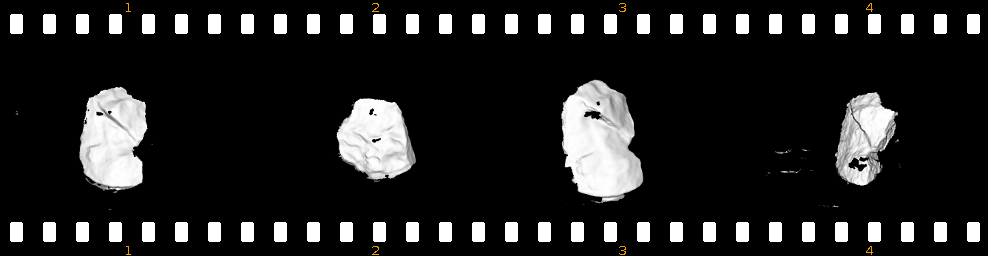
\includegraphics[width=0.45\textwidth]{filmstrips/rock.png}}}&
		\bmvaHangBox{\fbox{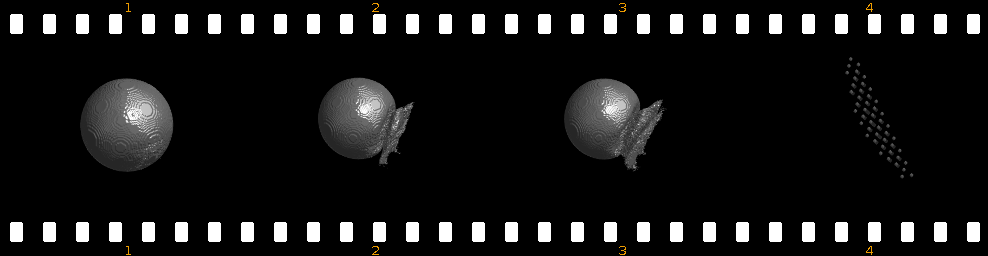
\includegraphics[width=0.45\textwidth]{filmstrips/rock_s3d_large.png}}}
	\end{tabular}
	\caption{
		Quarterly interval snapshots of the Rock reconstruction using \textbf{(L)} our method, and \textbf{(R)} the one proposed by Ren et~al.~\cite{Ren2013} with a large shape prior.
	}
	\label{fig:rockComparisonLarge}
\end{figure}

\begin{figure}[!h]
	\centering
	\begin{tabular}{cc}
		\bmvaHangBox{\fbox{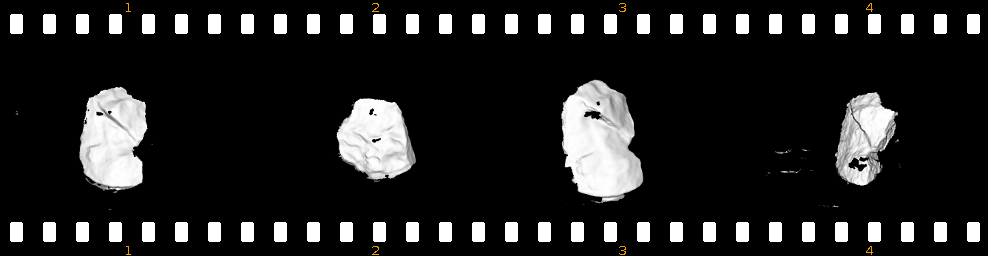
\includegraphics[width=0.45\textwidth]{filmstrips/rock.png}}}&
		\bmvaHangBox{\fbox{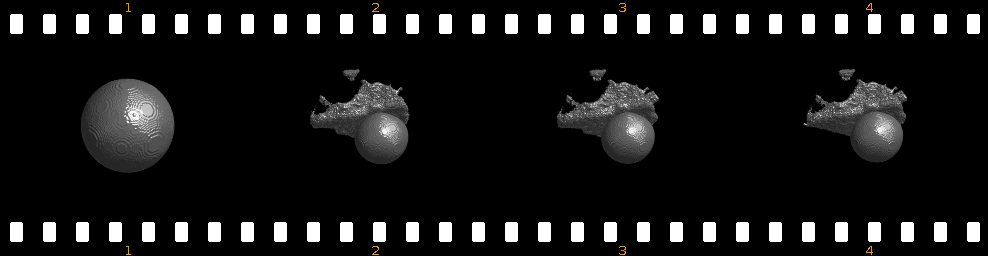
\includegraphics[width=0.45\textwidth]{filmstrips/rock_s3d_small.png}}}
	\end{tabular}
	\caption{
		Quarterly interval snapshots of the Rock reconstruction using \textbf{(L)} our method, and \textbf{(R)} the one proposed by Ren et~al.~\cite{Ren2013} with a small shape prior.
	}
	\label{fig:rockComparisonSmall}
\end{figure}

\section{Robustness to Noisy Probability Maps}
In this section we demonstrate robustness to instantaneously noisy and erroneous probability maps by showing clean reconstructions when the corresponding probability map for the 
current given frame has noise. Two sequences where this is particularly noteworthy are the \textit{DinoHead} and \textit{Rock} sequences. The examples of this for the \textit{DinoHead}
sequence can be seen in figure \ref{fig:dinoHeadMaps}. For the \textit{Rock} sequence, refer to figure \ref{fig:rockHeadMaps}.

\begin{figure}[!h]
	\centering
	\begin{tabular}{ccc}
		\bmvaHangBox{\fbox{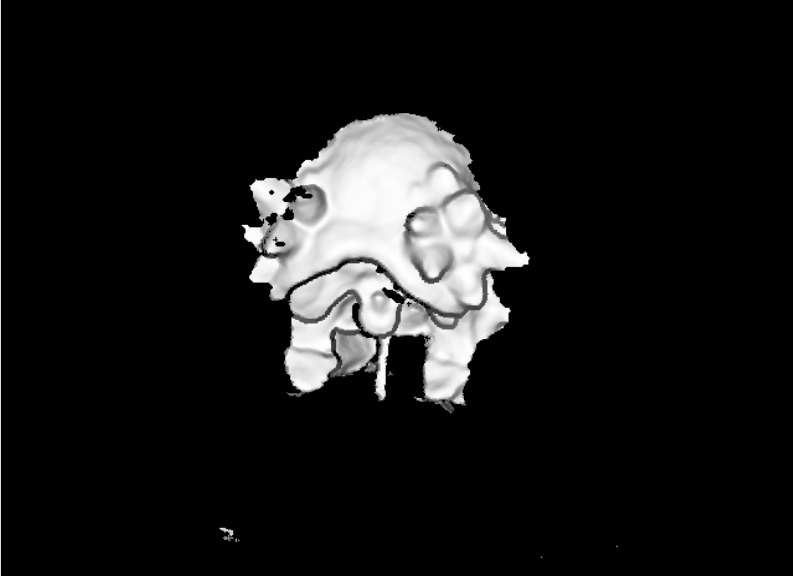
\includegraphics[width=0.25\textwidth]{rendered_frames/dino/rendering_1.png}}}&
		\bmvaHangBox{\fbox{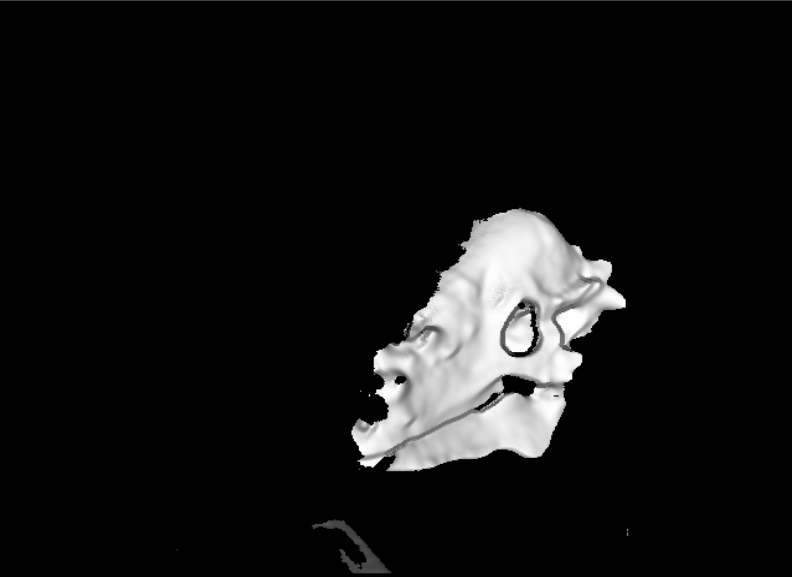
\includegraphics[width=0.25\textwidth]{rendered_frames/dino/rendering_2.png}}}&
		\bmvaHangBox{\fbox{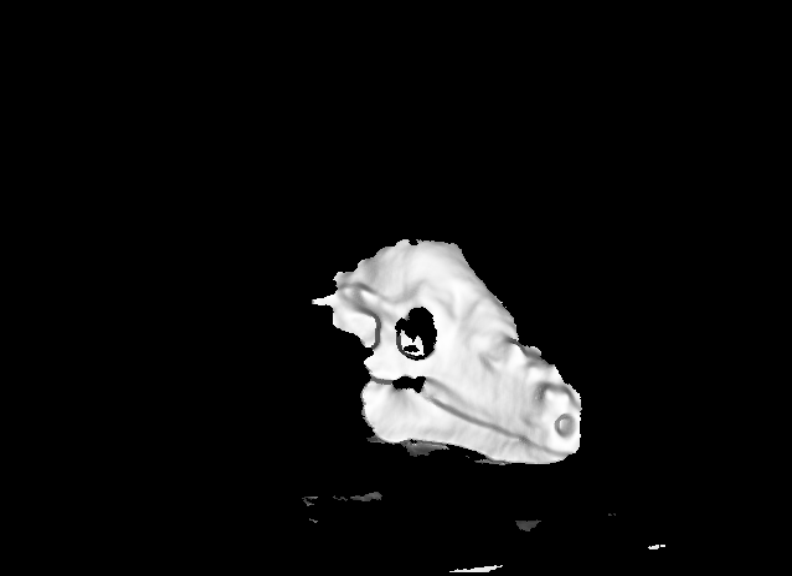
\includegraphics[width=0.25\textwidth]{rendered_frames/dino/rendering_3.png}}}\\
		\bmvaHangBox{\fbox{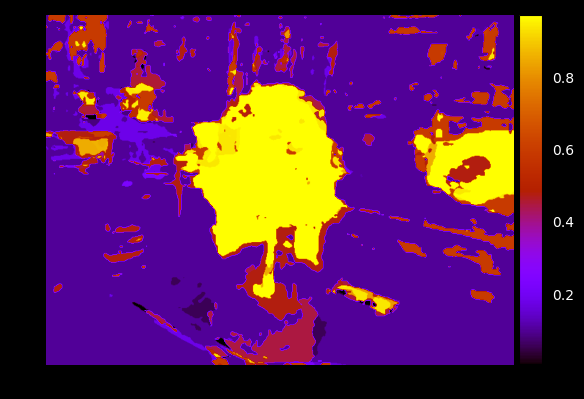
\includegraphics[width=0.25\textwidth]{rendered_frames/dino/heatmap_1.png}}}&
		\bmvaHangBox{\fbox{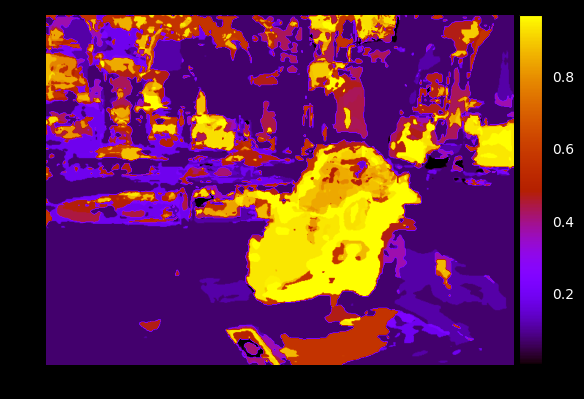
\includegraphics[width=0.25\textwidth]{rendered_frames/dino/heatmap_2.png}}}&
		\bmvaHangBox{\fbox{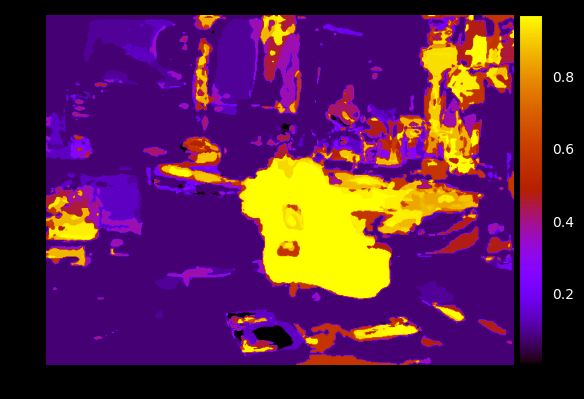
\includegraphics[width=0.25\textwidth]{rendered_frames/dino/heatmap_3.png}}}
	\end{tabular}
	\caption{
		Three reconstruction snapshots of the \textit{DinoHead} sequence and their associated probability maps.
	}
	\label{fig:dinoHeadMaps}
\end{figure}

\begin{figure}[!h]
	\centering
	\begin{tabular}{ccc}
		\bmvaHangBox{\fbox{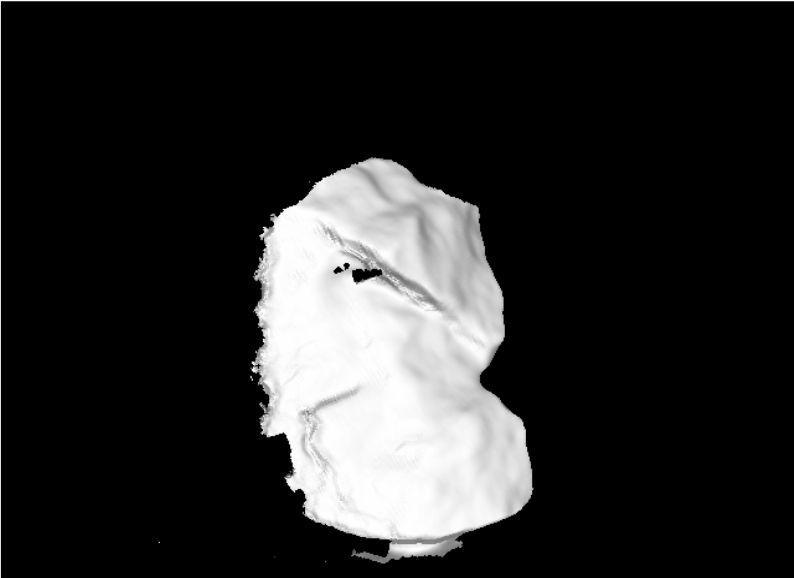
\includegraphics[width=0.25\textwidth]{rendered_frames/rock/rendering_1.png}}}&
		\bmvaHangBox{\fbox{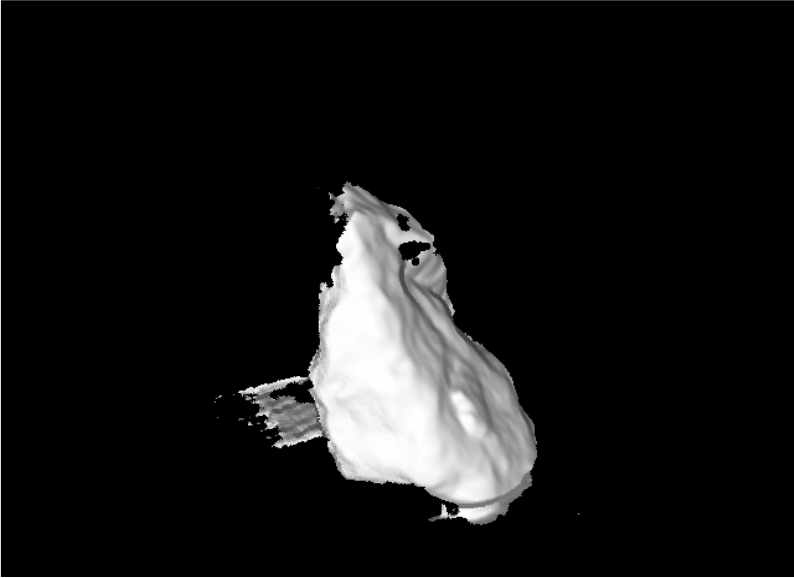
\includegraphics[width=0.25\textwidth]{rendered_frames/rock/rendering_2.png}}}&
		\bmvaHangBox{\fbox{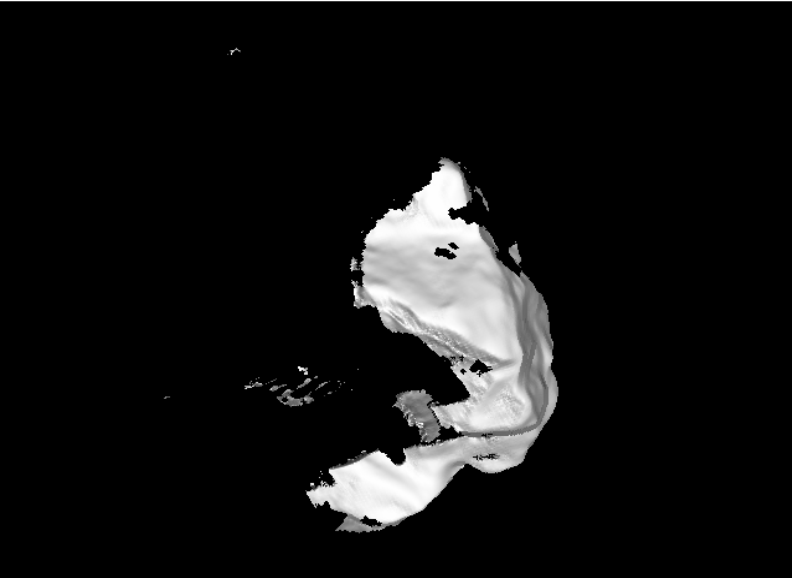
\includegraphics[width=0.25\textwidth]{rendered_frames/rock/rendering_3.png}}}\\
		\bmvaHangBox{\fbox{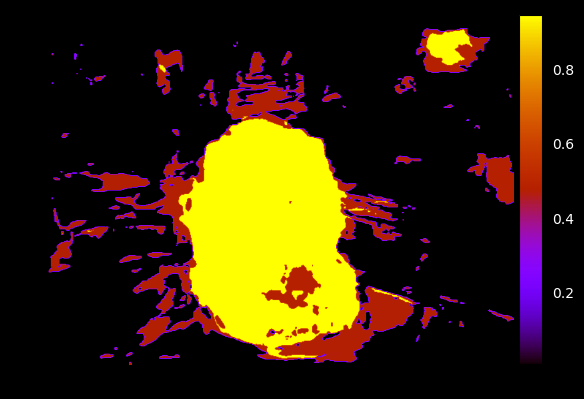
\includegraphics[width=0.25\textwidth]{rendered_frames/rock/heatmap_1.png}}}&
		\bmvaHangBox{\fbox{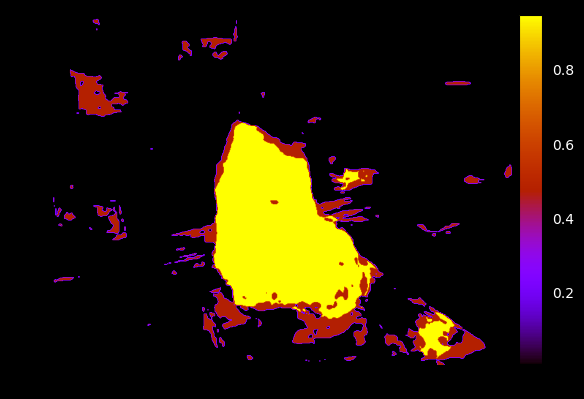
\includegraphics[width=0.25\textwidth]{rendered_frames/rock/heatmap_2.png}}}&
		\bmvaHangBox{\fbox{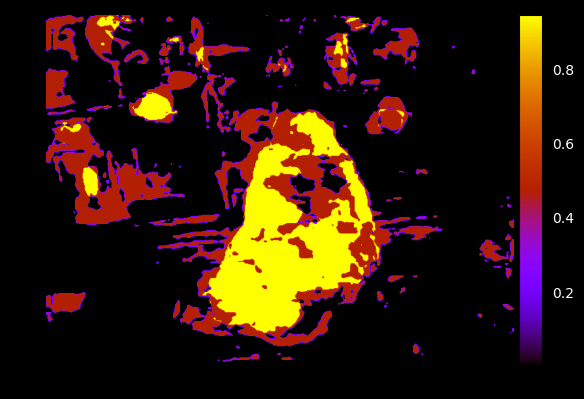
\includegraphics[width=0.25\textwidth]{rendered_frames/rock/heatmap_3.png}}}
	\end{tabular}
	\caption{
		Three reconstruction snapshots of the \textit{Rock} sequence and their associated probability maps.
	}
	\label{fig:rockHeadMaps}
\end{figure}

\section{Tracking Object Motion}
In addition to the reconstruction of the objects presented in the main paper and these supplementary materials, an experiment was performed in which the motion 
of a head is successfully tracked using only the geometry of the face. Quarterly snapshots are shown in figure \ref{fig:headTracking}.
\begin{figure}[!h]
	\centering
	\begin{tabular}{c}
		\bmvaHangBox{\fbox{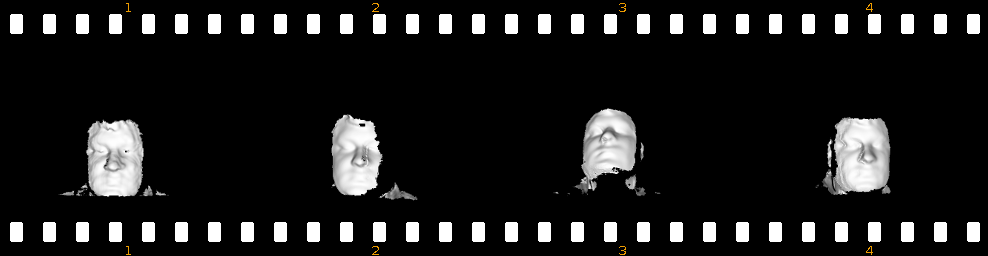
\includegraphics[width=0.45\textwidth]{filmstrips/face.png}}}
	\end{tabular}
	\caption{
		Quarterly interval snapshots of a face being reconstructed and tracked.
	}
	\label{fig:headTracking}
\end{figure}

\bibliography{bibliography}

\end{document}
